\documentclass{article}
\usepackage[UTF8]{ctex}
\usepackage{amsfonts}
\usepackage{amsmath}
\usepackage{float}
\usepackage{graphicx}
\usepackage{subcaption}
\usepackage{url}

\newcommand{\Bezier}{B\'ezier}%Bézier

\usepackage{color}

% paragraph
\setlength{\parindent}{0pt}
\setlength\parskip{\baselineskip}
\renewcommand{\baselinestretch}{1.2}

\begin{document}
	
	% 标题
	\title{《计算机辅助几何设计》作业}
	\author{ID号: 048  \qquad  姓名: 郑涛}  %递交作业时填上ID号和姓名
	\date{2024年12月19日}
	\maketitle
	\section{问题描述}
	本次实验目的是实现Tutte参数化,在老师的代码基础上实现Tutte参数化的算法。
	\section{程序思路说明}
	实验思想是用加权重心思想,由边缘的点加权生成内部的点。首先用findBoundary函数得到边缘点列,记为$B(i),i$为边缘点列在所有点列中的下标,将边缘点列映射到一个平面中去,本次实验用的是将边缘点列均匀映射到单位圆周上,其余每个点用与其相邻的点的平均加权表示线性映射到单位圆内。\\
	根据如上思想构造如下方程组:
	\begin{equation*}
		\begin{pmatrix}
			&1 &0 &\dotsb &-\frac{1}{k_{1}} &\dotsb  &0\\
			&0 &1 &\dotsb &-\frac{1}{k_{2}} &\dotsb  &0\\
			&\vdots & & & &  &\vdots \\
			&0 &\dotsb &1 &\dotsb  &0& \\
			&\vdots & & & &  &\vdots \\
			&0 &\dotsb &-\frac{1}{k_{n}} &\dotsb  &0& 1
		\end{pmatrix}
		\begin{pmatrix}
			u_{1}\\
			u_{2}\\
			\vdots\\
			u_{i}\\
			\vdots\\
			u_{n}
		\end{pmatrix}
		=
		\begin{pmatrix}
			a_{1}\\
			a_{2}\\
			\vdots\\
			a_{i}\\
			\vdots\\
			a_{n}
		\end{pmatrix}
	\end{equation*}
	其中,$u_{i}$和$a_{i}$为二维点,若第i个点在边缘,$a_{i}=q(i)$,且系数矩阵中$A(i,i)=1,A(i,j)=0(j\neq i)$,否则$a_{i}=0$,系数矩阵第i行中:
	$$
	A(i,j)=
	\left\{
	\begin{matrix}
		&1-\frac{1}{k_{i}}  &j=i\\
		&-\frac{1}{k_{i}}   &\mbox{下标为}i,j\mbox{所代表的点相邻}\\
		&0                  &others
	\end{matrix}
	\right .
	$$
	解得的$u_{i}$即为映射到单位圆内的点。
	\section{编译环境}
	本代码用Visual Studio2022编译
	\section{结果展示}
	\begin{figure}[H]
		\centering
		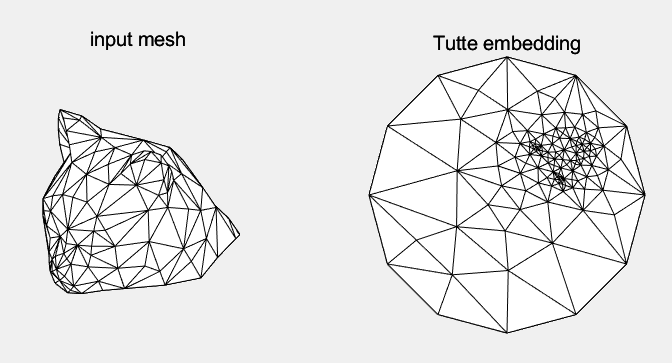
\includegraphics[scale=0.9]{result}
		\caption{}
		\label{fig:result}
	\end{figure}
	\section{实验结果分析}
	实现了Tutte参数化,有时间会尝试更多参数化方法。
\end{document}